% QuAM-xLSTM: journal manuscript (target: ACM TALLIP). Format-neutral draft in the article class;
% move into the journal template (acmart, acmsmall) once the format is confirmed.
% Compile: pdflatex main; bibtex main; pdflatex main; pdflatex main   (or upload the folder to Overleaf)
% All numbers come from paper/numbers.json, reports/*.json (scripts/paper_numbers.py,
% scripts/significance.py, scripts/unseen_aspects.py, scripts/journal_tables.py).
\documentclass[11pt]{article}
\usepackage[a4paper,margin=2.5cm]{geometry}
\usepackage[T1]{fontenc}
\usepackage[utf8]{inputenc}
\usepackage{lmodern}
\usepackage{microtype}
\usepackage{graphicx}
\usepackage{booktabs}
\usepackage{multirow}
\usepackage{amsmath,amssymb}
\usepackage{bm}
\usepackage{xcolor}
\usepackage[numbers,sort&compress]{natbib}
\usepackage[hidelinks]{hyperref}
\usepackage{tikz}
\usetikzlibrary{positioning,arrows.meta,fit,calc}
\usepackage{setspace}
\onehalfspacing

\newcommand{\pmstd}[2]{#1{\scriptsize$\pm$#2}}
\newcommand{\quam}{QuAM-xLSTM}

\title{Read Once, Query by Name: Aspect-Name Queries over an xLSTM Matrix Memory for
Aspect-Based Sentiment Analysis of Bangla, Banglish and English Reviews}

\author{First Author$^{1}$ \and Second Author (Supervisor)$^{1}$\\[2pt]
\small $^{1}$Department of Computer Science and Engineering, Daffodil International University, Dhaka, Bangladesh\\
\small \texttt{email@domain}}
\date{}

\begin{document}
\maketitle

% =========================================================================
\begin{abstract}
Aspect-based sentiment analysis (ABSA) of South Asian e-commerce reviews has to handle Bangla,
romanised Bangla (Banglish) and English, often mixed in a single review, and product categories
whose aspect inventories keep changing. We present \quam{}, a model that encodes a review once,
together with its product category, with a frozen multilingual encoder and a bidirectional xLSTM,
and answers every aspect by querying the final mLSTM matrix memory with the aspect name, combined
with a per-aspect scorer on pooled encoder states. Because published baselines on these data are
not directly comparable, we re-train fine-tuned BanglaBERT, fine-tuned XLM-R and a frozen-encoder
classifier on identical splits with the same metric code and validation-based threshold
selection. Tuned in this way, the baselines reach a strict aspect--sentiment pair F1 of 57.9
(BanglaBERT) and 62.1 (XLM-R) on EComReviews-BD, far above the 45.0 previously reported, and we show
that the reported precision--recall profile is consistent with an untuned presence threshold.
\quam{} trains 10M parameters on a 4\,GB laptop GPU. It matches fine-tuned BanglaBERT on the standard
split (\pmstd{58.0}{0.9} vs.\ \pmstd{57.9}{0.3}; $p=0.39$), trails it by 2.3 points on a leakage-free
split, and is the best system on product categories unseen in training, where it improves over
fine-tuned BanglaBERT by 1.9 points ($p=0.012$), over a strong frozen-encoder classifier by 7.0
points and over fine-tuned XLM-R by 13.4 points ($p<0.001$), and detects unseen aspect names that the
classifiers cannot represent (detection F1 20.1 vs.\ 1.5--7.1). It also detects rare aspects far better
than the fine-tuned encoders. We release a leakage-free split (11.5\% of the standard test reviews
also occur in training) and a zero-shot split, and we report the first aspect-sentiment baselines
on the BABSA dataset (macro-F1 70.6 for fine-tuned BanglaBERT). Ablations show that the memory read
mainly improves overall-review sentiment (+4.9 macro-F1) rather than aspect detection.
\end{abstract}

\noindent\textbf{Keywords:} aspect-based sentiment analysis; Bangla; Banglish; code-mixing;
low-resource languages; xLSTM; matrix memory; zero-shot aspects; evaluation

% =========================================================================
\section{Introduction}

E-commerce platforms in Bangladesh, such as Daraz, collect large numbers of short product reviews.
They are written in Bangla script, in Banglish (Bangla written in the Latin alphabet), in English,
or in a mixture of these within one review. Code-mixed text of this kind is known to be difficult
for sentiment models \citep{patwa2020sentimix}. For sellers and platforms a single review-level
polarity is of limited use: they need to know \emph{which} aspects of a product (price, delivery,
battery, sound quality, \dots) are praised or criticised. This is the task of aspect-based
sentiment analysis \citep[ABSA;][]{pontiki2014semeval,pontiki2016semeval,zhang2023absasurvey}.

Two properties of this setting motivate our work. First, the aspect inventory is not fixed:
marketplaces add product categories, and with them aspect names that a model has never seen. A
classifier with one output unit per known aspect cannot score such aspects at all. Second,
computing budgets in the research groups that work on Bangla are often small; our experiments run
on a single laptop GPU with 4\,GB of memory.

A common way to use pretrained encoders for ABSA is to pair the review with each aspect and
classify the pair \citep{sun2019auxiliary}. This handles any aspect name, but re-encodes a review
once per aspect. Recent work argues for reading a text once and answering every aspect from a
shared representation \citep{xia2026dabs}. Recurrent models with \emph{matrix memories} make this
particularly natural. The mLSTM of xLSTM \citep{beck2024xlstm} stores a sequence as a sum of gated
key--value outer products, $\mathbf{C}_T=\sum_t w_t\,\mathbf{v}_t\mathbf{k}_t^\top$, which can later
be read with any query vector, including the embedding of an aspect name that never occurred in
training. If the query is the aspect name, the read returns what the review ``wrote'' under that
aspect.

This article studies whether this idea holds up against carefully tuned baselines. We ask four
research questions:
\begin{description}
  \itemsep0em
  \item[RQ1] How strong are standard encoders on EComReviews-BD when they are trained and evaluated
  under identical conditions?
  \item[RQ2] Can a model that reads a review once with a frozen encoder and queries a fixed-size
  xLSTM memory with aspect names match fine-tuned encoders on known aspects?
  \item[RQ3] Does querying by name generalise to product categories and aspect names that were not
  seen in training?
  \item[RQ4] What does the memory read contribute, and which design choices matter?
\end{description}

Our contributions are:
\begin{enumerate}
  \itemsep0em
  \item \textbf{\quam{}} (Section~\ref{sec:method}), an ABSA model that reads a review once and
  answers each aspect by querying the final mLSTM matrix memory with the aspect name, combined with
  a per-aspect scorer on pooled encoder states. It trains 10M parameters on a frozen XLM-R and fits
  a 4\,GB GPU.
  \item \textbf{A controlled comparison} (Sections~\ref{sec:setup} and~\ref{sec:results}). We
  re-train BanglaBERT, XLM-R and a frozen-encoder classifier on exactly our splits with the same
  metric code and threshold selection, test differences with a paired bootstrap, and show that the
  baselines are 13--17 points stronger than previously reported (RQ1).
  \item \textbf{Where name-based querying helps} (RQ2, RQ3). \quam{} matches fine-tuned BanglaBERT on
  the standard split, trails it slightly without train--test overlap, and is the best system on
  unseen product categories and the only one that detects unseen aspect names to a useful degree.
  \item \textbf{Cleaner evaluation resources} (Section~\ref{sec:data}). We show that 11.5\% of the
  standard test reviews also occur in the training set, and release a leakage-free split, a
  zero-shot category split, and the first aspect-sentiment baselines on BABSA \citep{rohman2025babsa}.
  \item \textbf{Ablations and negative results} (Section~\ref{sec:ablation}, RQ4). The memory read
  alone is a weaker and less stable aspect detector than a pooled classifier; it mainly improves
  overall-review sentiment. Several plausible additions did not help.
\end{enumerate}
The code, the split definitions and all run configurations are available to reviewers and will be
released upon publication.

% =========================================================================
\section{Related Work}
\label{sec:related}

\subsection{Aspect-based sentiment analysis}
ABSA was popularised by the SemEval shared tasks on laptop and restaurant reviews
\citep{pontiki2014semeval,pontiki2016semeval}; \citet{zhang2023absasurvey} give a recent survey of
the many sub-tasks. Early neural models used aspect-conditioned attention over LSTM states
\citep{wang2016atae} or deep memory networks that attend repeatedly over word memories with the
aspect as the query \citep{tang2016memnet}. With pretrained Transformers \citep{vaswani2017attention,
devlin2019bert}, ABSA was often cast as sentence-pair classification by constructing an auxiliary
sentence from the aspect \citep{sun2019auxiliary}. Closest to our setting of predefined aspect
categories, \citet{schmitt2018joint} predict the presence and polarity of all categories jointly
in one model, and \citet{hu2019can} constrain attention so that multiple aspects of the same
sentence attend to different words. Large language models perform well on simple sentiment tasks
but lag behind small models trained on in-domain data on complex tasks that require structured
sentiment information, such as ABSA, while they excel in few-shot settings
\citep{zhang2024llmsentiment}. DABS \citep{xia2026dabs} encodes a sentence once into a
depth-organised Transformer representation and reads it with lightweight aspect-specific readouts.
Our work shares this single-pass goal; it differs in that the read-out operates on a recurrent
\emph{matrix memory} of fixed size, and in that the aspect is given by its name, so that new
aspects can be queried without new parameters.

\subsection{xLSTM, linear attention and recurrent alternatives}
xLSTM \citep{beck2024xlstm} extends the LSTM \citep{hochreiter1997lstm} with exponential gating and
two new cells: the sLSTM, a scalar memory with memory mixing, and the mLSTM, a matrix memory with a
covariance update rule. xLSTM 7B \citep{beck2025xlstm7b} scales the mLSTM to a large language model
and introduces, among other changes, a soft-cap on the gate pre-activations that we adopt. The
mLSTM is closely related to linear attention \citep{katharopoulos2020transformers} and to fast
weight programmers \citep{schlag2021fastweights}, which also store key--value associations in a
matrix that is read by queries. RWKV \citep{peng2023rwkv}, RetNet \citep{sun2023retnet} and
state-space models such as Mamba \citep{gu2023mamba} are further recurrent alternatives to
attention.

xLSTM has recently been applied to ABSA. AF-MAT \citep{lawan2025afmat} targets English benchmarks
(SemEval-2014 and Twitter): the aspect representation gates the mLSTM memory updates, a
flip-and-fuse block processes reversed sequences, and the final representation is mean-pooled over
tokens for each sentence--aspect pair. GateMABSA \citep{lawan2025gatemabsa} uses specialised mLSTMs
for multimodal (text and image) ABSA on English tweets. In both, the aspect \emph{modulates how the
sequence is written} into memory, so each sentence--aspect pair needs its own pass. In our model the
aspect is a \emph{query that reads} the finished memory, so one encoding serves all aspects. To our
knowledge, no prior work answers aspects by querying the final mLSTM memory, and no prior xLSTM ABSA
work covers Bangla or Banglish.

\subsection{Sentiment analysis for Bangla and code-mixed text}
Early Bangla ABSA datasets were small and covered only a few aspects
\citep{rahman2018banglaabsa,masum2020banabsa}. Sentence-level Bangla sentiment has received more
attention, including noisy social-media text \citep{islam2021sentnob} and the BLP-2023 shared task
\citep{hasan2023blp}. BanglishRev \citep{shamael2024banglishrev} provides large-scale Bangla,
English and code-mixed product reviews with ratings but without aspect labels, and the SentiMix
shared task \citep{patwa2020sentimix} studied sentiment in Hindi--English and Spanish--English
code-mixed tweets. Bangla-specific encoders such as BanglaBERT \citep{bhattacharjee2022banglabert}
and multilingual encoders such as mBERT \citep{devlin2019bert} and XLM-R \citep{conneau2020xlmr} are
the usual baselines. Two recent datasets make aspect-level work on Bangla possible at scale.
EComReviews-BD \citep{haque2026ecomreviews} provides 20,685 Daraz reviews in Bangla, Banglish and
English with aspect-level labels across 19 product categories, and reports fine-tuned Transformer
baselines. BABSA \citep{rohman2025babsa} provides about 16k Bangla texts from many domains with
aspect terms and their sentiment, annotated with high inter-annotator agreement (Cohen's
$\kappa\geq0.84$); the release itself reports no model results, and we are not aware of published
aspect-sentiment results on it.

% =========================================================================
\section{Method}
\label{sec:method}

\begin{figure}[t]
\centering
\resizebox{\textwidth}{!}{%
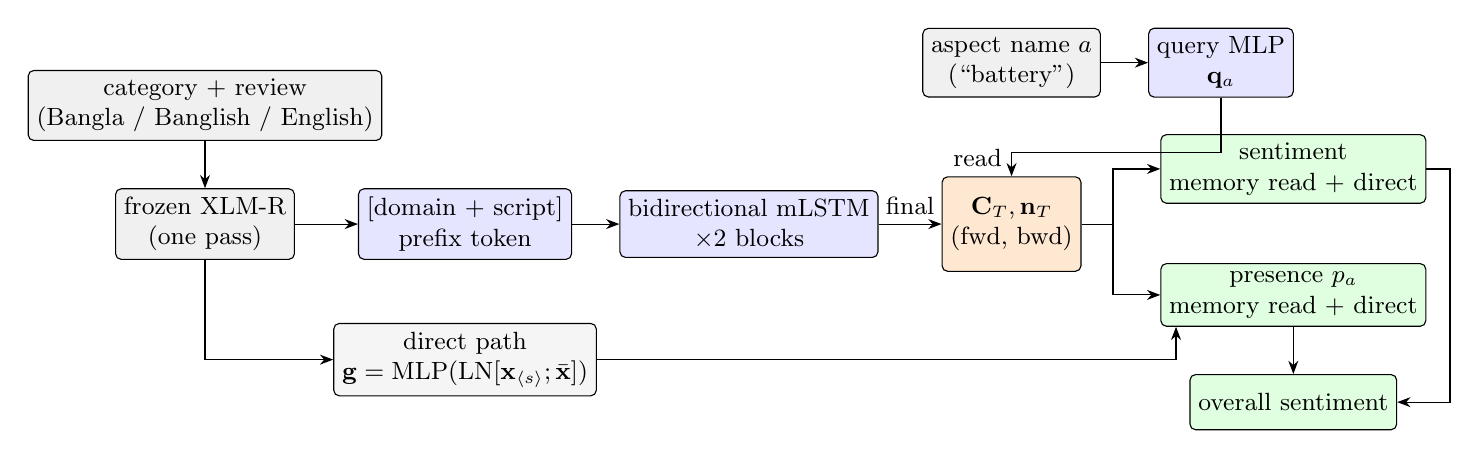
\begin{tikzpicture}[
  font=\small, >=Stealth,
  box/.style={draw, rounded corners=2pt, align=center, minimum height=7mm, inner sep=3pt},
  enc/.style={box, fill=gray!12},
  rnn/.style={box, fill=blue!10},
  mem/.style={box, fill=orange!18, minimum width=16mm, minimum height=12mm},
  head/.style={box, fill=green!12},
]
  \node[enc] (txt) {category + review\\(Bangla / Banglish / English)};
  \node[enc, below=6mm of txt] (xlmr) {frozen XLM-R\\(one pass)};
  \node[rnn, right=8mm of xlmr] (pre) {[domain + script]\\prefix token};
  \node[rnn, right=6mm of pre, minimum width=30mm] (bi) {bidirectional mLSTM\\$\times 2$ blocks};
  \node[mem, right=8mm of bi] (C) {$\mathbf{C}_T,\mathbf{n}_T$\\(fwd, bwd)};
  \node[box, fill=gray!8, below=8mm of pre] (g) {direct path\\$\mathbf{g}=\mathrm{MLP}(\mathrm{LN}[\mathbf{x}_{\langle s\rangle};\bar{\mathbf{x}}])$};
  \node[enc, above=10mm of C] (asp) {aspect name $a$\\(``battery'')};
  \node[rnn, right=6mm of asp] (q) {query MLP\\$\mathbf{q}_a$};
  \node[head, right=10mm of C, yshift=7mm] (sent) {sentiment\\memory read $+$ direct};
  \node[head, right=10mm of C, yshift=-9mm] (pres) {presence $p_a$\\memory read $+$ direct};
  \node[head, below=6mm of pres] (ov) {overall sentiment};
  \draw[->] (txt) -- (xlmr);
  \draw[->] (xlmr) -- (pre);
  \draw[->] (pre) -- (bi);
  \draw[->] (bi) -- node[above]{final} (C);
  \draw[->] (xlmr) |- (g);
  \draw[->] (asp) -- (q);
  \draw[->] (q) |- ($(C.north)+(0,3mm)$) -- node[left, pos=0.2]{read} (C.north);
  \draw[->] (C.east) -- ++(4mm,0) |- (sent.west);
  \draw[->] (C.east) -- ++(4mm,0) |- (pres.west);
  \draw[->] (g.east) -| ($(pres.south west)+(2mm,0)$);
  \draw[->] (sent.east) -- ++(3mm,0) |- (ov.east);
  \draw[->] (pres.south) -- (ov.north);
\end{tikzpicture}}
\caption{Overview of \quam{}. A review is encoded once together with its product category; every
aspect of the category is answered by a query into the final mLSTM matrix memory (one $O(d^2)$ read
per aspect, independent of review length), added to a per-aspect score on the pooled encoder states
$\mathbf{g}$ (a learned row for each known aspect plus a part computed from the aspect name).}
\label{fig:model}
\end{figure}

\subsection{Task definition}
A review $x$ belongs to a product category (domain) $c$ with aspect inventory $\mathcal{A}_c$. For
every $a\in\mathcal{A}_c$ the model predicts whether $a$ is mentioned (presence) and, if so, its
polarity; it also predicts the overall sentiment of the review (positive, neutral or negative). On
BABSA the aspects are given terms, and the task is their three-class sentiment. Figure~\ref{fig:model}
gives an overview of the model.

\subsection{Input encoding}
Each review is encoded once by a frozen XLM-R base \citep{conneau2020xlmr} as the sentence pair
(category name, review), i.e.\ \texttt{<s>} category \texttt{</s></s>} review \texttt{</s>}, so that
every token state is conditioned on the product category. Since every review belongs to exactly one
category, this is still a single encoder pass per review. Aspect names (e.g.\ \textit{click
buttons}) and category names are encoded by the same model and mean-pooled over their tokens. All
encoder outputs are computed once and cached, so training never runs the encoder.

XLM-R has a few outlier (``rogue'') feature dimensions \citep{timkey2021rogue}. In our data one
feature has mean 17.9 while the typical feature standard deviation is 0.08, which makes all aspect
embeddings nearly parallel (mean pairwise cosine 0.989). We therefore z-score every feature with
statistics from the training cache before the recurrent layers and the query network; without this
the presence head did not learn at all. A learned prefix token, the sum of a projection of the
category embedding and an embedding of the detected script (Bangla, English, Banglish, mixed), is
prepended to the token sequence.

\subsection{Bidirectional mLSTM}
The token sequence is projected to width $d{=}256$ and processed by $L{=}2$ pre-norm residual mLSTM
blocks \citep{beck2024xlstm} with up-projection to 512 and 4 heads of size 128. Each block is run
left-to-right and right-to-left. For one direction and head, with input gate $i_t$ (exponential)
and forget gate $f_t$ (sigmoid, computed in log space), the memory update is
\begin{align}
\mathbf{C}_t &= f_t\,\mathbf{C}_{t-1} + i_t\,\mathbf{v}_t\mathbf{k}_t^\top, &
\mathbf{n}_t &= f_t\,\mathbf{n}_{t-1} + i_t\,\mathbf{k}_t ,
\end{align}
computed in the stabilised parallel form with a running log-scale $m_t$. We soft-cap the gate
pre-activations with $15\tanh(\cdot/15)$, as in xLSTM 7B \citep{beck2025xlstm7b}; without it,
$e^{-m}$ overflowed and almost all batches produced non-finite gradients. Our implementation matches
the official parallel kernel to $9\times10^{-16}$ in double precision.

\subsection{Querying the memory with the aspect name}
After the last block we keep only $(\mathbf{C}_T,\mathbf{n}_T,m_T)$ of both directions. Each aspect
is mapped to a query $\mathbf{q}_a$ per head and direction by an MLP over its standardised name
embedding, and read exactly as the mLSTM reads at its own output step:
\begin{align}
\mathbf{r}_a &= \frac{\mathbf{C}_T\,\mathbf{q}_a}{\max\!\big(|\mathbf{n}_T^\top\mathbf{q}_a|,\,e^{-m_T}\big)},\\
\mu_a &= \log\!\big(|\mathbf{n}_T^\top\mathbf{q}_a| + e^{-m_T}\big) + m_T .
\end{align}
$\mathbf{r}_a$ is the value retrieved under key $\mathbf{q}_a$. $\mu_a$ equals
$\log(|\tilde{\mathbf{n}}_T^\top\mathbf{q}_a|+1)$ for the un-stabilised normaliser
$\tilde{\mathbf{n}}_T$, i.e.\ it measures how much key mass the review wrote in the direction of the
aspect; it is independent of the stabiliser and has a bounded gradient at
$\mathbf{n}^\top\mathbf{q}=0$. Reads from all heads and both directions are concatenated
($\mathbf{r}_a\in\mathbb{R}^{1024}$, $\bm{\mu}_a\in\mathbb{R}^{8}$, plus the log review length).
The memory per review is $2\times4\times128\times129 = 132{,}096$ numbers, independent of the review
length and of the number of aspects asked.

From the read, the sentiment logits are $\mathrm{MLP}_s(\mathrm{LN}(\mathbf{r}_a))$ and the presence
logit is $\mathrm{MLP}_p([\bm{\mu}_a;\mathbf{r}_a;\mathbf{u}_a])$, where
$\mathbf{u}_a=\mathrm{LN}(\mathbf{W}[\bar{\mathbf{h}};\mathbf{q}_a])$ adds the mean
$\bar{\mathbf{h}}$ of the final mLSTM token states. For EComReviews-BD, which has no neutral aspect
labels, the neutral logit is masked.

\subsection{Direct path with per-aspect scores}
A strong frozen-encoder classifier (Section~\ref{sec:setup}) owes much of its accuracy to two things
that the memory read lacks: the full 768-dimensional encoder states, and a separate output weight for
each aspect. We therefore add a direct path. The raw encoder states of the \texttt{<s>} token and
their mean over the sequence give
\begin{equation}
\mathbf{g}=\mathrm{GELU}\big(\mathbf{W}_g\,\mathrm{LN}([\mathbf{x}_{\langle s\rangle};\bar{\mathbf{x}}])\big)\in\mathbb{R}^{1024},
\end{equation}
and each aspect is scored as
\begin{equation}
s_a = \mathbf{e}_{\mathrm{id}(a)}^\top\mathbf{g} + \mathrm{MLP}([\mathbf{g};\mathbf{q}^{\mathrm{std}}_a]),
\label{eq:direct}
\end{equation}
with one such scorer for presence and one with three outputs for sentiment. $\mathbf{e}$ holds a
learned row for each of the 74 aspect names of EComReviews-BD, initialised to zero. An aspect name
that does not occur in training, or a BABSA aspect term, has the all-zero row and is scored by the
name-conditioned part alone. During training we replace the aspect id by the unknown id with
probability 0.2, so that the name-conditioned part stays useful. The direct scores are added to the
memory-read logits, and a linear map of $\mathbf{g}$ is added to the overall logits.

\subsection{Overall sentiment}
Each aspect receives a learned importance $w_a=\mathrm{softplus}(h([\mathbf{a};\mathbf{c}]))\,p_a$,
conditioned on the aspect and the category and weighted by its presence probability $p_a$. The
overall logits are
\begin{equation}
\mathrm{MLP}_o\Big(\sum_a w_a P_a^{+},\ \sum_a w_a P_a^{-},\ \sum_a w_a P_a^{0},\ \sum_a w_a\Big)
+\mathrm{MLP}_m(\mathbf{r}_{\textit{overall}}) + \mathbf{W}_o\mathbf{g},
\end{equation}
where $P_a$ are the aspect sentiment probabilities and $\mathbf{r}_{\textit{overall}}$ reads the
memory with the query ``overall opinion''.

\subsection{Training objective}
The loss is binary cross-entropy for presence over all aspects of the category, cross-entropy for
aspect sentiment on mentioned aspects, and $0.5\times$ cross-entropy for overall sentiment. BABSA only
annotates mentioned aspects, so for each review we add three aspect terms sampled from other
training reviews that do not occur in the text as negatives for presence.

\subsection{Cost}
A sentence-pair classifier \citep{sun2019auxiliary} encodes a review once per aspect, i.e.\
$|\mathcal{A}_c|$ encoder passes (about 13 on average in our test sets). \quam{} needs one encoder
pass per review, which can be cached, followed by one $O(d^2)$ memory read and one small scorer per
aspect. The fine-tuned baselines in Section~\ref{sec:setup} also need only one pass, because they
have an output row per aspect, but this ties them to a closed aspect inventory.

% =========================================================================
\section{Datasets and Splits}
\label{sec:data}

\begin{table}[t]
\centering\small
\begin{tabular}{lrr}
\toprule
 & EComReviews-BD & BABSA \\
\midrule
reviews / texts & 20,685 & 14,099 \\
median length (words) & 8 & 14 \\
categories / domains & 19 & 21 \\
aspects & 74 names & 16,968 (text, term) pairs \\
aspect labels & 18,513 pos / 6,414 neg & 5,479 pos / 5,858 neu / 5,631 neg \\
overall labels & 13,150 pos / 4,544 neu / 2,991 neg & -- \\
script: Bangla & 7,643 (36.9\%) & 13,882 (98.5\%) \\
script: English & 9,298 (45.0\%) & 31 \\
script: Banglish & 2,466 (11.9\%) & 60 \\
script: mixed & 1,237 (6.0\%) & 124 \\
train / val / test & 14,479 / 3,103 / 3,103 & 9,871 / 2,114 / 2,114 \\
\bottomrule
\end{tabular}
\caption{Dataset statistics after preprocessing. Scripts are detected automatically. BABSA duplicate
rows are merged per text; 20\% of its aspect terms do not occur verbatim in the text (implicit
aspects).}
\label{tab:data}
\end{table}

\subsection{EComReviews-BD}
EComReviews-BD \citep{haque2026ecomreviews} contains 20,685 Daraz reviews from 19 product categories
(Table~\ref{tab:data}). Each review carries a label in $\{-1,0,1\}$ for every aspect of its category,
where 0 means not mentioned; 91\% of the 267,948 (review, aspect) cells are not mentioned, and 26\% of
the mentioned aspects are negative. The aspect inventory has 74 distinct names; 42 of them occur in a
single category only. The dataset also contains NLLB \citep{nllb2022} English translations, aligned
for 19,943 reviews, which we use only in one ablation. We normalise text to Unicode NFC and detect the
script of each review from its characters.

\paragraph{Official split and train--test overlap.}
The official split (70/15/15, \texttt{random\_state}=42) is reproduced following the dataset
description. We use the published ratio, random seed and split sizes (14,479 / 3,103 / 3,103);
because the order in which the 19 category files are concatenated before splitting is not
specified, our test set may not contain exactly the same reviews as in the original paper. All
systems in our tables use our splits. We found that 358 of the 3,103 test texts (11.5\%) also occur in
the training set. They are mostly short generic reviews (median length two words, e.g.\ ``good
product''), so a model can score them by memorising training labels.

\paragraph{Grouped split.} We therefore also use a grouped split of the same sizes in which identical
normalised texts never cross split boundaries.

\paragraph{Zero-shot split.} To test generalisation to new product categories, the test set of the
zero-shot split consists of four categories never seen in training (Router, WebCam, Mini\_Printer and
CC\_Camera; 2,637 test reviews with 2,750 mentioned aspects, and 17,510 / 538 reviews for training
and validation). 18 of their aspect names never occur in
training, and these account for 956 of the 2,750 test mentions; the remaining aspect names (e.g.\
\textit{price}, \textit{quality}) also occur in other categories.

\subsection{BABSA}
BABSA \citep{rohman2025babsa} contains Bangla texts from 21 domains (book reviews, politics, religion,
food, \dots) with aspect terms and their three-class sentiment. We merge duplicate rows per text,
which gives 14,099 texts with 16,968 (text, term) pairs, and drop 43 conflicting aspect labels. 20\% of
the aspect terms do not occur verbatim in the text (implicit aspects). The release is sorted by label,
so shuffling before splitting is essential; we create a grouped 70/15/15 split stratified by domain
and label.

\subsection{Evaluation metrics}
Following \citet{haque2026ecomreviews}, the main metric on EComReviews-BD is \emph{strict pair}
precision, recall and F1: a prediction counts as correct only if a mentioned aspect is detected
\emph{and} its polarity is right. The original paper does not state how these scores are averaged; we
use micro-averaging over all (review, aspect) pairs. We also report detection F1, macro-F1 of
detection over aspect names (which weights rare aspects equally), polarity accuracy on gold-mentioned
aspects, and overall-sentiment macro-F1. For every system, the presence threshold is chosen on the
validation set from $\{0.05,0.10,\dots,0.95\}$ and applied unchanged to the test set. On BABSA we
report three-class sentiment accuracy and macro-F1 over gold aspect terms, separately for verbatim
and implicit terms.

% =========================================================================
\section{Experimental Setup}
\label{sec:setup}

\begin{table}[t]
\centering\small
\begin{tabular}{lccc}
\toprule
 & \quam{} & fine-tuned encoders & frozen encoder + MLP \\
\midrule
encoder & XLM-R base, frozen & BanglaBERT / XLM-R base & BanglaBERT / XLM-R base, frozen \\
input & (category, review) & (category, review) & (category, review) \\
trainable parameters & 10.0M & 110M / 86M$^\ast$ & 1.8M \\
optimiser & AdamW & AdamW & AdamW \\
learning rate & $10^{-3}$ & $2\times10^{-5}$ & $10^{-3}$ \\
weight decay & 0.05 & 0.01 & 0.01 \\
schedule & 5\% warm-up, cosine & 10\% warm-up, linear & 10\% warm-up, linear \\
batch size & 32 & 16 & 16 \\
epochs & 15 & $\leq$10 (patience 3) & $\leq$15 (patience 4) \\
model selection & best validation pair F1 & best validation pair F1 & best validation pair F1 \\
time per run (RTX 2050) & $\approx$12 min & $\approx$30 / 40 min & $\approx$10 min \\
\bottomrule
\end{tabular}
\caption{Training configurations on EComReviews-BD. All systems use the same losses (presence BCE,
sentiment CE, $0.5\times$ overall CE), bf16 autocast, gradient clipping at 1.0, maximum 256 tokens, and
the same validation-based threshold selection. $^\ast$XLM-R with frozen word embeddings and gradient
checkpointing to fit into 4\,GB.}
\label{tab:setup}
\end{table}

\paragraph{\quam{}.} Table~\ref{tab:setup} lists the training configuration. Dropout is 0.1. XLM-R
states are pre-computed once with a maximum of 256 tokens (24 texts are truncated), so a run takes
about 12 minutes on a single RTX 2050 laptop GPU with 4\,GB of memory (peak 1.9\,GB). We do not use
early stopping, because memory-based detection can start slowly (Section~\ref{sec:ablation}); the
epoch with the best validation pair F1 is selected.

\paragraph{Fine-tuned encoders.} BanglaBERT \citep{bhattacharjee2022banglabert} and XLM-R base
\citep{conneau2020xlmr} encode the pair (category, review). The \texttt{[CLS]} state feeds one
presence logit and one polarity pair per aspect (74 output rows) and a three-way overall head, trained
with the same losses as \quam{}. The learning rate of $2\times10^{-5}$ follows
\citet{haque2026ecomreviews}. To fit XLM-R into 4\,GB we freeze its word embeddings (86M of its 278M
parameters remain trainable) and use gradient checkpointing, which changes memory use but not the
computation. BanglaBERT is used with our NFC-normalised text but without its own normaliser.

\paragraph{Frozen-encoder classifier.} This baseline feeds
$\mathrm{LN}([\mathbf{x}_{\texttt{[CLS]}};\bar{\mathbf{x}}])$ of the frozen encoder through a 1024-unit
GELU layer to the same heads. It isolates what a simple head achieves on the same frozen features that
\quam{} uses.

\paragraph{BABSA baselines.} On BABSA the baselines classify the pair (aspect term, text) into three
classes from the \texttt{[CLS]} state (fine-tuned: up to 5 epochs, patience 2) or from the frozen
features through the same MLP (up to 15 epochs, patience 4), selected by validation macro-F1.

\paragraph{Seeds, ensembles and significance.} We report mean $\pm$ sample standard deviation over
three seeds (42, 1, 2) unless marked otherwise; because of compute limits, fine-tuned XLM-R and frozen
BanglaBERT were run with one seed. A \emph{seed ensemble} of \quam{} averages the three models'
probabilities \citep{lakshminarayanan2017ensembles}, with its threshold re-chosen on validation.
Differences in pair F1 are tested with a paired bootstrap over test reviews: we resample the 3,103
test reviews with replacement 10,000 times, compute the seed-averaged pair F1 of both systems on each
sample (2,637 reviews on the zero-shot split), and report the mean difference, its 95\% percentile interval and the fraction of samples in
which \quam{} is not better ($p$).

% =========================================================================
\section{Results}
\label{sec:results}

\begin{table}[p]
\centering\footnotesize
\setlength{\tabcolsep}{3.5pt}
\begin{tabular}{llrccccccc}
\toprule
split & model & trainable & pair P & pair R & \textbf{pair F1} & det.\ F1 & det.\ mF1 & pol.\ acc & overall F1 \\
\midrule
\multirow{8}{*}{official}
 & BanglaBERT, reported$^\dagger$       & 110M & 31.8 & 77.1 & 45.0 & -- & -- & -- & -- \\
 & BanglaBERT, fine-tuned               & 110M & \pmstd{62.4}{1.9} & \pmstd{54.0}{1.1} & \pmstd{57.9}{0.3} & \pmstd{62.1}{0.3} & \pmstd{15.4}{0.5} & \pmstd{89.4}{0.4} & \pmstd{78.4}{0.7} \\
 & XLM-R, fine-tuned$^1$                & 86M  & 67.7 & 57.3 & \textbf{62.1} & 67.5 & 17.2 & 89.2 & 78.1 \\
 & BanglaBERT, frozen + MLP$^1$         & 1.8M & 47.5 & 46.3 & 46.9 & 52.0 & 20.6 & 86.3 & 67.4 \\
 & XLM-R, frozen + MLP                  & 1.8M & \pmstd{60.4}{1.6} & \pmstd{56.8}{1.3} & \pmstd{58.6}{0.4} & \pmstd{66.3}{0.4} & \pmstd{35.4}{0.9} & \pmstd{85.8}{0.3} & \pmstd{67.5}{0.1} \\
 & \quam{}                              & 10M  & \pmstd{59.4}{0.5} & \pmstd{56.8}{2.2} & \pmstd{58.0}{0.9} & \pmstd{64.9}{1.1} & \pmstd{32.4}{2.4} & \pmstd{87.1}{0.2} & \pmstd{70.6}{0.7} \\
 & \quam{}, 3-seed ensemble             & 30M  & 59.4 & 58.9 & 59.2 & 65.9 & 34.1 & 87.7 & 71.6 \\
\midrule
\multirow{5}{*}{grouped}
 & BanglaBERT, fine-tuned               & 110M & \pmstd{61.4}{2.5} & \pmstd{54.9}{1.6} & \pmstd{58.0}{0.6} & \pmstd{61.8}{0.5} & \pmstd{17.4}{0.6} & \pmstd{90.1}{0.1} & \pmstd{77.5}{0.7} \\
 & XLM-R, fine-tuned$^1$                & 86M  & 63.9 & 60.1 & \textbf{61.9} & 66.9 & 21.3 & 88.8 & 76.2 \\
 & XLM-R, frozen + MLP                  & 1.8M & \pmstd{58.0}{2.4} & \pmstd{56.3}{2.1} & \pmstd{57.1}{0.1} & \pmstd{65.2}{0.1} & \pmstd{34.2}{1.6} & \pmstd{85.7}{0.3} & \pmstd{64.9}{0.4} \\
 & \quam{}                              & 10M  & \pmstd{59.0}{0.6} & \pmstd{52.6}{1.1} & \pmstd{55.6}{0.3} & \pmstd{62.8}{0.2} & \pmstd{28.6}{1.1} & \pmstd{86.4}{0.2} & \pmstd{69.2}{1.4} \\
 & \quam{}, ensemble                    & 30M  & 61.0 & 51.8 & 56.0 & 63.2 & 27.9 & 87.0 & 70.9 \\
\midrule
\multirow{5}{*}{zero-shot}
 & BanglaBERT, fine-tuned               & 110M & \pmstd{70.6}{5.9} & \pmstd{26.9}{1.4} & \pmstd{38.9}{0.7} & \pmstd{41.8}{1.0} & \pmstd{13.3}{1.0} & \pmstd{74.4}{0.9} & \textbf{\pmstd{63.3}{0.6}} \\
 & XLM-R, fine-tuned$^1$                & 86M  & 21.0 & 39.4 & 27.4 & 31.7 & 21.4 & 72.1 & 63.0 \\
 & XLM-R, frozen + MLP                  & 1.8M & \pmstd{57.4}{13.3} & \pmstd{24.5}{2.1} & \pmstd{33.8}{1.3} & \pmstd{37.7}{0.9} & \pmstd{16.7}{1.4} & \pmstd{73.5}{1.9} & \pmstd{58.9}{0.7} \\
 & \quam{}                              & 10M  & \pmstd{39.5}{2.1} & \pmstd{42.4}{1.1} & \textbf{\pmstd{40.9}{1.0}} & \pmstd{46.7}{0.5} & \pmstd{28.4}{1.2} & \pmstd{85.6}{0.7} & \pmstd{61.3}{0.6} \\
 & \quam{}, ensemble                    & 30M  & 38.1 & 44.0 & 40.8 & 46.7 & 29.5 & 86.5 & 61.2 \\
\bottomrule
\end{tabular}
\caption{EComReviews-BD test results. All rows except $^\dagger$ are trained and evaluated by us on
identical splits with the same metric code and validation-chosen threshold; mean$\pm$std over three
seeds, $^1$one seed. $^\dagger$Reported by \citet{haque2026ecomreviews} on their split (which may
differ, Section~\ref{sec:data}) without stated averaging. \emph{trainable}: trained parameters,
frozen encoders not counted; \emph{det.\ mF1}: detection macro-F1 over aspect names; \emph{pol.\ acc}:
polarity accuracy on gold-mentioned aspects.}
\label{tab:main}
\end{table}

\begin{table}[t]
\centering\small
\begin{tabular}{llccc}
\toprule
split & \quam{} vs. & $\Delta$ pair F1 & 95\% CI & $p$ \\
\midrule
official & BanglaBERT, fine-tuned & $+0.2$ & $[-1.0,\ 1.4]$ & 0.39 \\
official & XLM-R, frozen + MLP & $-0.5$ & $[-1.3,\ 0.3]$ & 0.90 \\
grouped & BanglaBERT, fine-tuned & $-2.3$ & $[-3.5,\ -1.2]$ & 1.00 \\
grouped & XLM-R, frozen + MLP & $-1.5$ & $[-2.2,\ -0.7]$ & 1.00 \\
zero-shot & BanglaBERT, fine-tuned & $+1.9$ & $[0.2,\ 3.6]$ & 0.012 \\
zero-shot & XLM-R, fine-tuned$^1$ & $+13.4$ & $[12.0,\ 14.9]$ & $<$0.001 \\
zero-shot & XLM-R, frozen + MLP & $+7.0$ & $[5.6,\ 8.4]$ & $<$0.001 \\
\bottomrule
\end{tabular}
\caption{Paired bootstrap tests over test reviews (10,000 samples; three seeds per system unless
marked, $^1$one seed; pair F1 averaged over seeds). $p$ is the fraction of samples in which \quam{} is not better than the
baseline.}
\label{tab:sig}
\end{table}

\subsection{RQ1: Baselines are much stronger than reported}
Table~\ref{tab:main} shows that, trained on the same split and with a validation-chosen threshold,
fine-tuned BanglaBERT reaches \pmstd{57.9}{0.3} pair F1 instead of the reported 45.0, and fine-tuned
XLM-R reaches 62.1. Even a frozen XLM-R with a one-layer MLP head reaches \pmstd{58.6}{0.4}. The
reported baselines have very high recall at low precision (77.1 / 31.8). The same profile appears
when the presence threshold of our own models is set too low: at a threshold of 0.1, our fine-tuned
BanglaBERT (seed 42) obtains P 29.6 / R 76.9 / F1 42.8 on our test set, and at 0.05 \quam{} obtains
P 29.5 / R 79.1 / F1 43.0 (Figure~\ref{fig:sweep}). At the default threshold of 0.5 BanglaBERT already
reaches 55.1, and at its validation-chosen threshold (0.35) 58.2. Since 91\% of the aspect cells are
absent, the presence threshold has a large effect on strict pair F1. We cannot verify how the
original baselines were thresholded, but these numbers show that the reported scores understate what
the same encoders achieve, and we compare only against our own runs.

\begin{figure}[t]
\centering
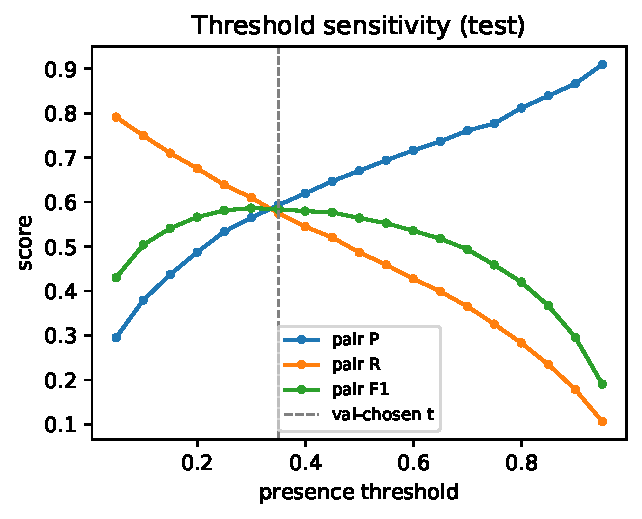
\includegraphics[width=0.48\textwidth]{figures/threshold_sweep.pdf}\hfill
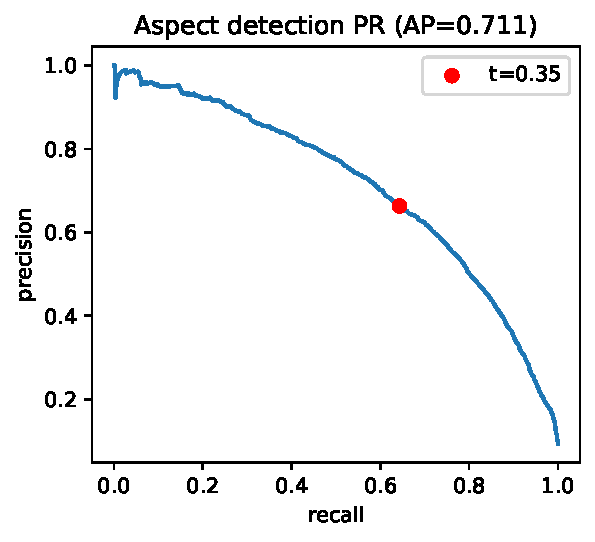
\includegraphics[width=0.48\textwidth]{figures/pr_eco_detection.pdf}
\caption{Left: pair and detection P/R/F1 of \quam{} as a function of the presence threshold (official
split, test, seed 42); a low threshold gives the high-recall, low-precision profile of the reported
baselines. Right: precision--recall curve of aspect detection.}
\label{fig:sweep}
\end{figure}

\subsection{RQ2: Known product categories}
On the official split, \quam{} (\pmstd{58.0}{0.9}; 59.2 as an ensemble) is on par with fine-tuned
BanglaBERT and with the frozen-encoder classifier (Table~\ref{tab:sig}; neither difference is
significant), while training 10M instead of 110M parameters. Without the train--test overlap (grouped
split) it trails both, by 2.3 and 1.5 points, and both differences are significant. Fine-tuned XLM-R is
the best system on seen categories (62.1 and 61.9, single runs): when the aspect inventory is known,
updating the encoder still pays off.

The systems differ beyond pair F1. The fine-tuned encoders are much better at overall-review sentiment
(78.4 vs.\ 70.6 macro-F1 for \quam{}) and slightly better at aspect polarity (89.4 vs.\ 87.1). The
frozen-encoder models, on the other hand, detect rare aspects far better: detection macro-F1 over
aspect names is 28.6--35.4 for \quam{} and the frozen classifier, but only 15.4--21.3 for the
fine-tuned encoders. Fine-tuning thus appears to fit the frequent aspects at the expense of rare ones
(Section~\ref{sec:analysis}).

\begin{table}[t]
\centering\small
\begin{tabular}{lcccc}
\toprule
 & \multicolumn{2}{c}{seen aspect names} & \multicolumn{2}{c}{unseen aspect names} \\
 & \multicolumn{2}{c}{(1,794 mentions)} & \multicolumn{2}{c}{(956 mentions)} \\
\cmidrule(lr){2-3}\cmidrule(lr){4-5}
model & det.\ F1 & pair F1 & det.\ F1 & pair F1 \\
\midrule
BanglaBERT, fine-tuned & \pmstd{57.5}{1.8} & \pmstd{53.8}{1.6} & \pmstd{1.5}{1.1} & \pmstd{0.6}{0.5} \\
XLM-R, fine-tuned$^1$ & \textbf{68.9} & \textbf{64.1} & 7.1 & 3.1 \\
XLM-R, frozen + MLP & \pmstd{52.9}{2.6} & \pmstd{47.7}{2.0} & \pmstd{1.5}{2.6} & \pmstd{1.0}{1.7} \\
\quam{} & \pmstd{62.2}{0.1} & \pmstd{55.2}{0.9} & \pmstd{20.1}{2.0} & \pmstd{16.3}{1.5} \\
\quam{} without memory & \pmstd{62.2}{1.1} & \pmstd{54.6}{0.3} & \textbf{\pmstd{21.1}{1.1}} & \textbf{\pmstd{17.0}{0.9}} \\
\bottomrule
\end{tabular}
\caption{Zero-shot split (four unseen product categories): test mentions split by whether the aspect
name occurs in training. Mean$\pm$std over three seeds, $^1$one seed.}
\label{tab:unseen}
\end{table}

\subsection{RQ3: Unseen product categories and aspect names}
On four product categories never seen in training, \quam{} is the best system with \pmstd{40.9}{1.0}
pair F1: 1.9 points above fine-tuned BanglaBERT (95\% CI $[0.2,3.6]$, $p=0.012$), 7.0 above the
frozen-encoder classifier ($[5.6,8.4]$, $p<0.001$) and 13.4 above fine-tuned XLM-R ($p<0.001$). The
baselines fail in two different ways. Fine-tuned BanglaBERT and the frozen classifier become very
conservative on new categories (recall 24.5--26.9), whereas fine-tuned XLM-R over-predicts (precision
21.0). \quam{} keeps a balanced profile (P 39.5, R 42.4) and a much higher polarity accuracy (85.6 vs.\
72.1--74.4). Fine-tuned BanglaBERT remains best on overall sentiment (63.3).

Table~\ref{tab:unseen} separates the test mentions by whether the aspect name occurs in training. The
classifiers cannot represent the 18 unseen names, since their output rows for these aspects were never
trained, and detect them with F1 of 1.5--7.1. For fine-tuned XLM-R, these untrained rows fire often: it
predicts 3,802 mentions of unseen names against 956 gold mentions, which explains its low overall
precision. \quam{} detects unseen names with F1 \pmstd{20.1}{2.0}. On the seen aspect names of the new
categories, fine-tuned XLM-R is clearly best (64.1 pair F1), followed by \quam{} (\pmstd{55.2}{0.9}) and
fine-tuned BanglaBERT (\pmstd{53.8}{1.6}); \quam{}'s overall advantage therefore comes from the unseen
names and from not misfiring on them. The variant without the memory is about as good, so this
advantage comes from scoring aspects by their name (Equation~\ref{eq:direct} and the query network),
not from the memory specifically. Unseen aspect names remain hard for all systems.

\begin{table}[t]
\centering\small
\begin{tabular}{lrccc}
\toprule
model & trainable & accuracy & macro-F1 & implicit macro-F1 \\
\midrule
BanglaBERT, fine-tuned & 110M & \textbf{\pmstd{70.5}{0.3}} & \textbf{\pmstd{70.6}{0.4}} & \textbf{\pmstd{66.2}{0.6}} \\
XLM-R, fine-tuned$^1$ & 86M & 67.9 & 67.8 & 63.0 \\
XLM-R, frozen + MLP & 1.8M & \pmstd{62.0}{0.7} & \pmstd{61.9}{0.4} & \pmstd{55.4}{1.4} \\
\quam{} & 10M & \pmstd{63.2}{0.2} & \pmstd{63.1}{0.3} & \pmstd{57.8}{1.9} \\
\quam{}, ensemble & 30M & 63.8 & 63.6 & 58.6 \\
\bottomrule
\end{tabular}
\caption{First aspect-sentiment baselines on BABSA (grouped split, test, 2,570 aspect terms, of which
510 are implicit). Mean$\pm$std over three seeds, $^1$one seed.}
\label{tab:babsa}
\end{table}

\subsection{BABSA}
Table~\ref{tab:babsa} gives, to our knowledge, the first aspect-level sentiment results on BABSA. Here
the aspect terms are open-ended, so the per-aspect rows of \quam{} are unused and it scores aspects by
name only. Fine-tuned BanglaBERT is clearly best (\pmstd{70.6}{0.4} macro-F1), which is expected for an
almost purely Bangla-script dataset (98.5\%) and a Bangla-specific encoder. Among the frozen-encoder
models, \quam{} improves over the classifier by 1.2 points. Implicit aspect terms are harder for every
model (4--7 points), and neutral is the hardest class (Figure~\ref{fig:cm}, right).

% =========================================================================
\section{Ablations and Negative Results}
\label{sec:ablation}

\begin{table}[t]
\centering\small
\begin{tabular}{lcc}
\toprule
model (grouped split) & pair F1 & overall F1 \\
\midrule
\multicolumn{3}{l}{\textit{three seeds}} \\
\quad \quam{}                      & \textbf{\pmstd{55.6}{0.3}} & \textbf{\pmstd{69.2}{1.4}} \\
\quad direct path only (no memory) & \pmstd{55.3}{0.2} & \pmstd{64.3}{0.3} \\
\quad v1: memory read only$^\ddagger$  & \pmstd{43.3}{7.3} & \pmstd{69.5}{0.6} \\
\quad v1: memory + pooled tokens$^\ddagger$ & \pmstd{47.2}{2.3} & \pmstd{68.4}{0.3} \\
\quad v1: mean pooling only$^\ddagger$ & \pmstd{45.8}{1.4} & \pmstd{66.9}{0.7} \\
\quad v1: memory, tied query init.$^\ddagger$ & \pmstd{41.4}{4.9} & \pmstd{69.6}{0.6} \\
\midrule
\multicolumn{3}{l}{\textit{seed 42: building up \quam{} from v1}} \\
\quad v1 + direct path (z-scored) & 52.9 & 64.1 \\
\quad \quad + category-paired encoding & 54.0 & 69.9 \\
\quad \quad \quad batch 16, weight decay 0.01 & 51.6 & 63.7 \\
\quad \quad \quad \quad and no aspect-id dropout & 53.4 & 67.1 \\
\quad \quad + raw direct features (= \quam{}) & 55.2 & 68.3 \\
\midrule
\multicolumn{3}{l}{\textit{v1, seed 42, early stopping}} \\
\quad presence from $\bm{\mu}$ only & 29.2 & 68.6 \\
\quad no domain/script prefix & 40.8 & 67.3 \\
\quad 3 mLSTM blocks         & 38.4 & 68.5 \\
\quad + sLSTM block (m-m-s-m) & 30.0 & 56.0 \\
\quad + cross-lingual consistency & 39.1 & 68.9 \\
\bottomrule
\end{tabular}
\caption{Ablations (grouped split, test). $^\ddagger$v1: our first model, without the direct path and
with the review encoded alone. Rows from single runs are indicative only.}
\label{tab:ablation}
\end{table}

\subsection{RQ4: What the memory contributes}
Table~\ref{tab:ablation} separates the two paths of \quam{}. Removing the memory read leaves aspect
detection essentially unchanged (55.3 vs.\ 55.6 pair F1 on the grouped split; 40.3 vs.\ 40.9 on the
zero-shot split) but costs 4.9 points of overall-sentiment macro-F1 (3.6 on zero-shot). The memory is
therefore most useful as a summary of the whole review, while aspect detection is driven by the pooled
encoder states and the per-aspect scorer.

Querying the memory alone (v1) was a weaker and unstable detector. Across seeds its pair F1 ranged from
35.1 to 49.3: inspecting the training curves, the weaker seeds spend many epochs with a nearly constant
presence loss before detection starts to improve, while mean pooling does not show this plateau. This
is why we train for a fixed number of epochs without early stopping. Averaged over seeds as an ensemble,
the memory-only v1 model was better than pooling (49.3 vs.\ 47.6), so the memory does carry aspect
information, but it is harder to optimise.

\subsection{From v1 to \quam{}}
Our first model (v1) read only the memory and encoded the review alone; on the grouped split it reached
\pmstd{47.2}{2.3}, almost ten points below the frozen-encoder classifier. Three changes closed most of
this gap (seed 42): adding the direct path (52.9), encoding the review together with its category
(54.0; this is also worth 3.1 points for the frozen classifier, 57.2 vs.\ 54.1), and feeding raw
rather than z-scored encoder states to the direct path (55.2). Matching the baselines' batch size and
weight decay lowered results (51.6). In that setting, removing aspect-id dropout recovered 1.8 points
(53.4), so the dropout, which keeps the name-based scorer useful for unseen aspects, may cost some
accuracy on seen aspects; we keep it because unseen categories are the setting where \quam{} is most
useful.

\subsection{What did not help}
\textit{Tied query initialisation}, which starts each aspect query as the key that the memory would
write for the aspect name, raised the presence signal at initialisation (AUROC of the raw read
0.44$\rightarrow$0.55) but did not improve final results. \textit{Per-aspect thresholds} tuned on
validation lowered test pair F1 (45.4$\rightarrow$42.9 for v1), because validation and test differ for
rare aspects. \textit{Cross-lingual consistency} between a review and its NLLB translation hurt
(39.1), plausibly because machine translations of Banglish are noisy. Adding an \textit{sLSTM block}
lowered results (30.0) and made training 4.5$\times$ slower; these runs used early stopping with patience
4, which interacts with the slow-start behaviour above, so the sLSTM result may be pessimistic. The
\textit{domain/script prefix} helped by 4.6 points, and a third mLSTM block did not help.

% =========================================================================
\section{Analysis}
\label{sec:analysis}

\begin{figure}[t]
\centering
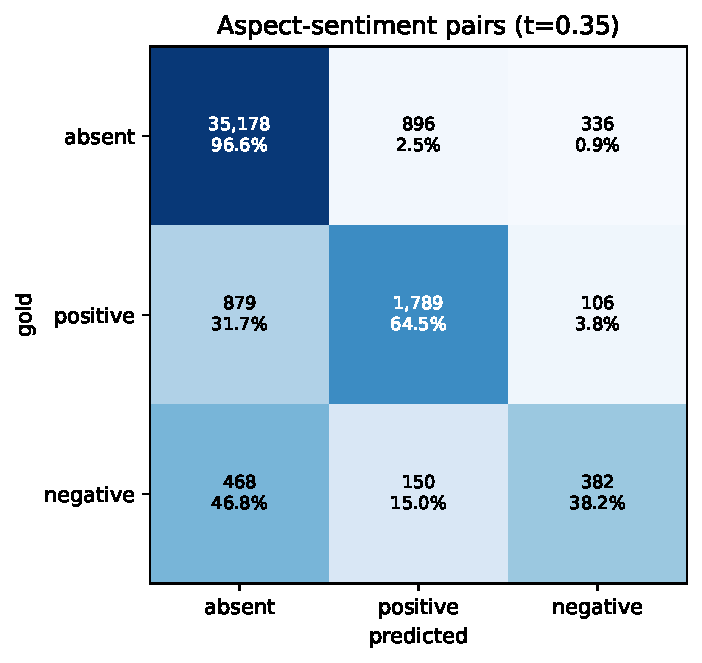
\includegraphics[width=0.46\textwidth]{figures/cm_eco_joint.pdf}\hfill
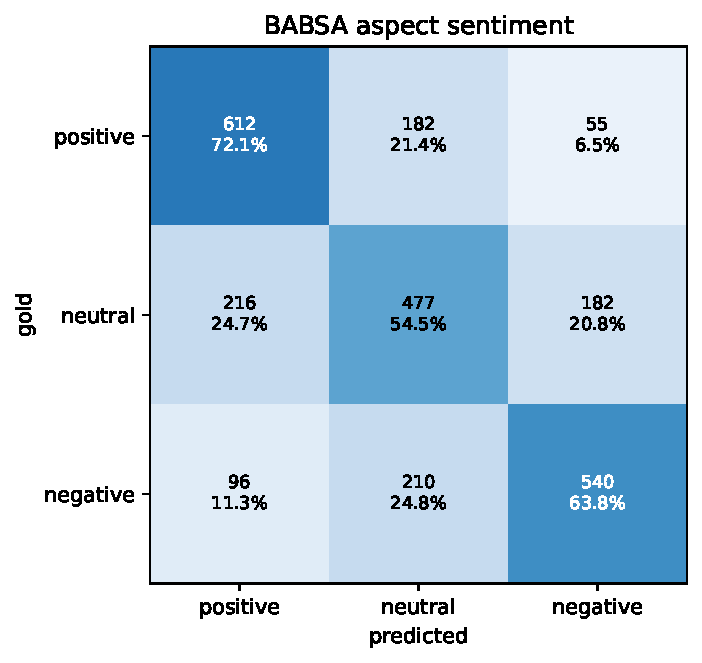
\includegraphics[width=0.46\textwidth]{figures/cm_babsa.pdf}
\caption{Test confusion matrices of \quam{} (rows: gold; percentages are row-normalised). Left:
EComReviews-BD aspect--sentiment pairs, official split, seed 42. Right: BABSA aspect sentiment, seed
42.}
\label{fig:cm}
\end{figure}

\paragraph{Missed negative aspects.}
Figure~\ref{fig:cm} (left) shows that 47\% of mentioned negative aspects are predicted as absent,
against 32\% of positive ones. Negative aspects are less frequent (26\% of mentioned aspects), and we
hypothesise that complaints are more often expressed without naming the aspect; verifying this
requires a manual study that we leave to future work. When a negative aspect is detected, its polarity
is right in 72\% of cases (382 of 532), against 94\% for positive aspects (1,789 of 1,895).

\paragraph{Rare aspects.}
Detection quality depends strongly on how often an aspect occurs in training (Figure~\ref{fig:freq}):
on the grouped split, detection F1 is 68.8 for the 10 aspects with ${\geq}500$ training mentions, 45.5
for the 25 aspects with 50--499 and 23.0 for the 39 aspects with fewer than 50 (seed 42). Because more
than half of the aspects are rare, macro-F1 over aspect names stays far below micro F1 for every
system, and the fine-tuned encoders suffer most (Table~\ref{tab:main}).

\begin{figure}[t]
\centering
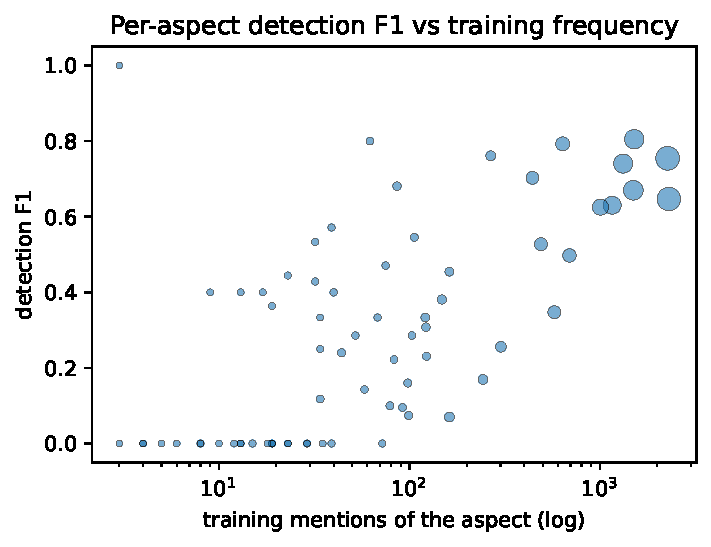
\includegraphics[width=0.6\textwidth]{figures/aspect_f1_vs_freq.pdf}
\caption{Per-aspect detection F1 of \quam{} against the number of training mentions (grouped split,
seed 42; marker size = test mentions).}
\label{fig:freq}
\end{figure}

\begin{table}[t]
\centering\small
\begin{tabular}{lcccc}
\toprule
model (official split) & English & Bangla & mixed & Banglish \\
\midrule
BanglaBERT, fine-tuned & 60.0 & 56.4 & 56.8 & 55.9 \\
XLM-R, fine-tuned$^1$ & \textbf{64.5} & \textbf{59.8} & \textbf{63.2} & \textbf{60.2} \\
XLM-R, frozen + MLP & 61.9 & 56.3 & 57.7 & 54.0 \\
\quam{} & 61.8 & 55.7 & 56.3 & 53.0 \\
\midrule
test reviews & 1,416 & 1,137 & 189 & 356 \\
\bottomrule
\end{tabular}
\caption{Pair F1 by script of the review (official split, test; mean over three seeds, $^1$one seed).}
\label{tab:script}
\end{table}

\paragraph{Scripts.}
Table~\ref{tab:script} breaks pair F1 down by script. All systems are best on English and worst on
Banglish, which has no standard spelling and is under-represented in the encoders' pretraining data.
The frozen-encoder systems lose most on Banglish (53.0--54.0, against 55.9 for fine-tuned BanglaBERT
and 60.2 for fine-tuned XLM-R), which suggests that adapting the encoder matters most for romanised
text. Since our model's frozen encoder is the main limitation here, combining name-based querying with
a fine-tuned encoder is a natural next step.

\paragraph{Efficiency.}
With pre-computed encoder states, the \quam{} head processes about 1,500 test reviews per second
(0.7\,ms per review including all aspect reads, 0.5\,GB peak GPU memory) on the RTX 2050. These numbers
exclude the frozen encoder, which runs once per review and is shared by all aspects and all training
epochs. A \quam{} training run takes about 12 minutes, against about 30 (BanglaBERT) and 40 minutes
(XLM-R) for fine-tuning on the same GPU, and its peak training memory (1.9\,GB) leaves room on a 4\,GB
card where fine-tuning XLM-R required freezing the embeddings.

% =========================================================================
\section{Discussion}
\label{sec:discussion}

\paragraph{When to use which model.}
Our results suggest a simple rule. When the product categories and their aspect inventories are known
and enough labelled data exist, a fine-tuned encoder with one output per aspect is the most accurate
choice; fine-tuned XLM-R was best on all seen-category splits, and fine-tuned BanglaBERT on the
Bangla-only BABSA. When new categories appear, or many aspects are rare, a model that scores aspects by
their name is preferable: \quam{} was the best system on unseen categories, detected unseen aspect
names that the classifiers could not represent, and detected rare aspects better than the fine-tuned
encoders. A fine-tuned encoder still handles the known aspects of a new category best, which suggests
combining the two: a fine-tuned encoder for the known inventory and name-based scoring for new names. \quam{} also needs far less compute, because the encoder runs once per review and is not
trained.

\paragraph{Role of the matrix memory.}
The initial hypothesis of this work was that querying the final xLSTM memory with the aspect name would
be a strong aspect detector by itself. This was only partly confirmed. The memory does carry aspect
information (as an ensemble the memory-only model outperformed mean pooling), but it is harder to
optimise and is outperformed by a pooled per-aspect scorer. In the final model, the memory mainly
improves overall-review sentiment (+4.9 macro-F1), where summarising the whole review matters. We
report this negative result because it constrains how matrix memories should be read: as a summary
that complements pooled features rather than as a replacement for them.

\paragraph{Evaluation practice.}
Two findings concern evaluation more than modelling. First, a substantial part of the gap between a
new model and published baselines can come from the baselines' training and thresholding rather than
from the model, so baselines should be re-run under identical conditions and with a tuned decision
threshold. Second, 11.5\% of the standard test reviews also occur in training. \quam{} scores 2.4
points higher on the official than on the grouped split (58.0 vs.\ 55.6), while fine-tuned BanglaBERT
scores the same on both (57.9 vs.\ 58.0). The two test sets differ in more than the overlap, but the
comparison between the systems changes from a tie to a significant difference, so we recommend
reporting the grouped split alongside the official one.

\paragraph{Threats to validity.}
Our reproduction of the official split may not select exactly the same rows as the original paper.
Some baselines were run with a single seed, and XLM-R was fine-tuned with frozen word embeddings to fit
into 4\,GB, which may slightly underestimate it. BanglaBERT was used without its own normaliser. The
significance tests account for test-set sampling and average over three seeds, but do not fully capture
training variance. The zero-shot split contains only four categories and 18 unseen aspect names. The
v1 ablations at the bottom of Table~\ref{tab:ablation} are single runs with early stopping. Both
datasets come from Bangladesh, and we did not test other languages or domains.

% =========================================================================
\section{Conclusion}
\label{sec:conclusion}

We studied aspect-based sentiment analysis of Bangla, Banglish and English e-commerce reviews with
\quam{}, a model that reads a review once and answers aspects by querying an xLSTM matrix memory with
the aspect name, combined with a per-aspect scorer on pooled encoder states. Trained and evaluated
under identical conditions, standard encoders are far stronger on EComReviews-BD than previously
reported, and fine-tuned XLM-R is the best system when the aspect inventory is known (RQ1). With a
frozen encoder and 10M trained parameters, \quam{} matches fine-tuned BanglaBERT on the standard split
but trails it without train--test overlap (RQ2). It is the best system on unseen product categories
and the only one that detects unseen aspect names to a useful degree, an advantage that comes from
scoring aspects by name (RQ3). The memory read mainly improves overall-review sentiment, not
detection (RQ4). We also release a leakage-free and a zero-shot split and the first aspect-sentiment
baselines on BABSA. Future work should combine name-based querying with a fine-tuned encoder, improve
the detection of unseen aspect names and of implicitly expressed negative aspects, and extend the
evaluation to further low-resource and code-mixed settings.

% =========================================================================
\section*{Data and Code Availability}
EComReviews-BD is available under CC BY 4.0 and BABSA under CC BY-NC-SA 4.0 from their original
publications. Our code, the split definitions (as lists of review identifiers) and the configurations
of all runs reported here will be released upon publication.

\section*{Ethics Statement}
Both datasets are public; the BABSA licence restricts our use of it to non-commercial research. The
reviews may contain names of sellers or products, but no personal data were collected by us. ABSA
systems can be used to filter or rank reviews; errors that systematically miss negative aspects
(Section~\ref{sec:analysis}) could favour sellers, so deployments should be audited for this.

\section*{Use of AI Assistants}
An AI assistant was used to help write code and to draft parts of the manuscript. The authors designed
the study, reviewed and verified all code, experiments, numbers and citations, and take full
responsibility for the content.

\section*{Acknowledgements}
% To be completed for the final version.

\bibliographystyle{plainnat}
\bibliography{references}

\end{document}
